\section{Experiments}
\label{sec:experiments}

We systematically compare \cls{}, \cwm{}, and \traj{} across two representative code LLM families, two complexity levels, and multiple seeds to characterize the formulation landscape for neural code verification.

\subsection{Experimental Setup}
\label{sec:setup}

\paragraph{Datasets.}
\emph{Function-level}: mutated variants from HumanEval~\cite{chen2021humaneval} and MBPP~\cite{austin2021mbpp} (five mutation types), labels verified by execution. 19,076 samples (train 15,290 / val 1,896 / test 1,890; pass:fail $\approx$ 52:48, majority baseline 51.75\%).
\emph{Repo-level}: per-test instances from SWE-bench Verified~\cite{chowdhury2024swebenchverified} mutants. ${\sim}$70K training samples; val ($n{=}9{,}335$) and test ($n{=}9{,}784$) have zero problem overlap (majority baseline 72.96\%). Val-based checkpoint selection follows standard practice~\cite{jimenez2024swebench}; runs with NaN validation loss (due to truncated targets exceeding 2,048-token limits) default to the final epoch checkpoint (Appendix~\ref{app:hyperparams}). Qwen3 \cwm{} runs show early overfitting (best at ${\sim}$6\% of training); checkpoint details in Appendix~\ref{app:hyperparams}.

\paragraph{Models and training.}
We fine-tune Qwen3-4B and Qwen3-8B~\cite{qwen2025qwen3} with LoRA~\cite{hu2022lora} (rank 16, 3 epochs) across five seeds (3 bfloat16, 2 NF4 4-bit~\cite{dettmers2024qlora}). DeepSeek-Coder-6.7B~\cite{guo2024deepseekcoder} serves as a cross-model check (2 seeds). Our \cwm{} baseline uses LoRA fine-tuning for matched comparison, not the 32B CWM~\cite{meta2025cwm}. Zero-shot baselines use Qwen3-8B and Qwen3-32B (NF4). Full hyperparameters in Appendix~\ref{app:hyperparams}; prompts in Appendix~\ref{app:prompts}.

\paragraph{Statistics.}
Equivalence uses Two One-Sided Tests (TOST)~\cite{schuirmann1987tost} with $\pm$2\pp{} margin; seed-level paired analysis (df${=}$4 for 5-seed, df${=}$2 for 3-seed) treats each training seed as the unit of replication. Holm-Bonferroni correction~\cite{holm1979} controls family-wise error across the five primary comparisons (Table~\ref{tab:holm}). Confidence intervals use clustered bootstrap~\cite{davison1997bootstrap} (114 problem clusters, 10K resamples); intraclass correlation coefficient (ICC)~\cite{shrout1979icc} quantifies within-problem correlation. Bayesian Region of Practical Equivalence (ROPE) and mixed-effects regression supplement these tests. Full statistical power analysis in Appendix~\ref{app:power}.


\subsection{Function-Level Results}
\label{sec:func_results}

Table~\ref{tab:main_results} reports function-level results across formulations and model families.

\begin{table}[t]
\centering
\small
\caption{Function-level per-test accuracy on HumanEval+MBPP ($n{=}1{,}890$). Mean $\pm$ std over 5 seeds (Qwen3) or 2 seeds (DeepSeek). Seeds 42/123/456: bfloat16; 789/0: NF4. DeepSeek: $n{=}2$ seeds; std reported for descriptive comparison, not inferential. \traj{}\textsuperscript{$\star$} evaluated on 1,032-sample subset (447 matched variants). All prompting baselines use NF4 4-bit quantization. \textsuperscript{$\star$}Training configuration differs (\S\ref{sec:repo}).}
\label{tab:main_results}
\setlength{\tabcolsep}{6pt}
\renewcommand{\arraystretch}{1.0}
\begin{tabular}{llcc}
\toprule
\textbf{Method} & \textbf{Model} & \textbf{Seeds} & \textbf{Accuracy (\%)} \\
\midrule
\multicolumn{4}{l}{\emph{Qwen3 (primary)}} \\
\cls{} (fine-tuned) & 4B & 5 & \textbf{88.43 $\pm$ 0.78} \\
\cwm{} (fine-tuned) & 4B & 5 & \underline{87.19 $\pm$ 0.37} \\
\traj{}\textsuperscript{$\star$} (fine-tuned) & 4B & 5 & 86.30 $\pm$ 0.97 \\
\midrule
\multicolumn{4}{l}{\emph{DeepSeek-Coder (cross-model consistency check)}} \\
\cls{} (fine-tuned) & 6.7B & 2 & \textbf{86.85 $\pm$ 0.11} \\
\cwm{} (fine-tuned) & 6.7B & 2 & \underline{86.83 $\pm$ 1.49} \\
\traj{}\textsuperscript{$\star$} (fine-tuned) & 6.7B & 2 & 84.16 $\pm$ 1.30 \\
\midrule
\multicolumn{4}{l}{\emph{Prompting baselines}} \\
0-shot & 8B (Qwen3) & 1 & 60.53 \\
0-shot & 14B (Qwen3) & 1 & 66.24 \\
0-shot & 6.7B (DeepSeek) & 1 & 63.02 \\
Zero-shot LLM-as-judge & 8B (Qwen3) & 1 & 64.40 \\
Zero-shot LLM-as-judge & 6.7B (DeepSeek) & 1 & 56.56 \\
Zero-shot LLM-as-judge & 32B (NF4) & 1 & 71.69 \\
3-shot in-context learning & 8B (Qwen3) & 1 & 60.42 \\
3-shot in-context learning & 14B (Qwen3) & 1 & 73.12 \\
3-shot in-context learning & 6.7B (DeepSeek) & 1 & 59.95 \\
\midrule
Majority (pass) & --- & --- & 51.75 \\
\bottomrule
\end{tabular}
\end{table}

All three formulations achieve comparable accuracy on Qwen3-4B: \cls{} 88.43\%, \cwm{} 87.19\%, \traj{} 86.30\% (Table~\ref{tab:main_results}). The \cls{}--\cwm{} gap (0.02--1.24\pp{}) is within seed noise across both families; the \cls{}--\traj{} gap (2.13--2.69\pp{}) exceeds the $\pm$2\pp{} equivalence margin on DeepSeek-Coder (\S\ref{sec:equivalence}). Zero-shot baselines confirm that repo-level verification requires fine-tuning (35--36\pp{} gains) and that formulation choice matters only at repo level (\cls{} outperforms \cwm{} by 18--26\pp{}).


\subsection{Scaling Behavior}
\label{sec:scaling}

Beyond overall accuracy, we examine whether formulation ranking is stable across model sizes. Table~\ref{tab:scaling} compares all three formulations at 4B, 8B, and 14B. The 4B and 8B rows use seeds 42 and 123; the 14B row uses seeds 42, 123, and 456. All rows use bfloat16 inference.

\begin{figure}[t]
\centering
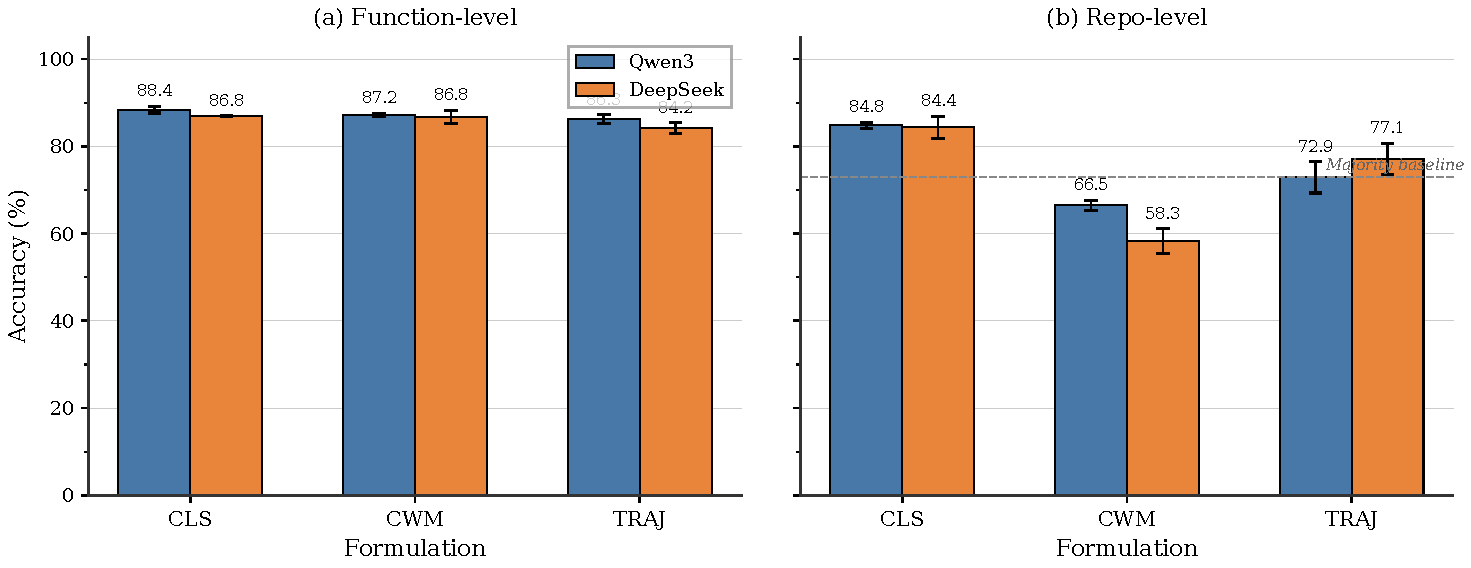
\includegraphics[width=0.82\columnwidth]{figures/paper/figure2_v3.pdf}
\caption{Function-level accuracy scaling (4B--14B). CLS and CWM accuracy with shaded gap region; $y$-axis does not start at zero. The \cls{}--\cwm{} gap shows a non-monotonic pattern: 1.32\pp{} at 4B, widening to 2.62\pp{} at 8B, then narrowing to 0.43\pp{} at 14B (3 seeds).}
\label{fig:scaling_gap}
\end{figure}

\cls{} and \traj{} both scale positively from 4B to 8B (+1.27\pp{} and +2.13\pp{} respectively), while \cwm{} remains flat ($-$0.03\pp{}). At 8B, the ranking is \cls{} (89.94) $>$ \traj{} (87.70) $>$ \cwm{} (87.33). The \cls{}--\cwm{} gap widens from 1.32\pp{} at 4B to 2.62\pp{} at 8B (Figure~\ref{fig:scaling_gap}); clustered bootstrap on the 3-seed superset (42, 123, 456 for \cls{}/\cwm{}) yields $p = 0.0066$ (95\% CI $[1.80, 2.71]$), which confirms the widening is not a sampling artifact.

At 14B (3 seeds), all three formulations converge in point estimates: \cls{} 89.93$\pm$0.80\%, \cwm{} 89.50$\pm$0.67\%, \traj{} 88.86$\pm$0.77\%. The maximum pairwise gap (\cls{}--\traj{}) narrows from 3.11\pp{} at 4B to 1.07\pp{} at 14B, within the $\pm$2\pp{} margin. Seed-level TOST (df${=}$2) is inconclusive in both pairs ($p{=}0.076$ for \cls{}--\cwm{}, $p{=}0.187$ for \cls{}--\traj{}), reflecting the low power of 3-seed comparisons; Bayesian ROPE provides moderate support ($P(\text{ROPE}){=}0.887$ and $0.780$; Appendix~\ref{app:bayesian_rope}). \cwm{}'s delayed scaling onset (flat 4B--8B, then +2.17\pp{} at 14B) and \traj{}'s decelerating convergence (+2.13\pp{} at 8B, +1.16\pp{} at 14B) are both consistent with capacity-dependent convergence at function level.

\paragraph{Baseline scaling.} Prompting baselines remain well below fine-tuning: the best result (14B 3-shot, 73.12\%) is 16.82\pp{} below fine-tuned \cls{} at 8B. Only \cls{} scales positively across both complexity levels; \traj{} shows negligible repo-level scaling (72.92\% at 4B, 73.61\% at 8B).


\subsection{Function-Level Equivalence}
\label{sec:equivalence}

We test pairwise equivalence on 523 variant-level instances across five seeds.\footnote{Seeds 789/0 use NF4 inference; the remaining three use bfloat16. Restricting to bfloat16 only: \cls{}--\cwm{} remains significant ($p{<}0.05$); \cls{}--\traj{} yields $p{=}0.128$.} Our Smallest Effect Size of Interest (SESOI) threshold of $\pm$2\pp{}~\cite{lakens2017,wellek2010} is domain-motivated but not pre-registered: at 85--88\% accuracy, 2\pp{} corresponds to ${\sim}$2--3 problems out of 114, below practitioner-relevant differences and consistent with between-seed variation (0.37--0.97\pp{} std). Within-problem predictions are correlated (ICC $= 0.191$, design effect [DEFF] $= 3.97$~\cite{moulton1990}); confidence intervals use clustered bootstrap (\S\ref{sec:setup}). Sensitivity analysis shows \cls{}--\cwm{} equivalence is robust across margins down to $\pm$1.63\pp{} (Table~\ref{tab:tost_sensitivity}, Figure~\ref{fig:tost_sensitivity}); \cls{}--\traj{} equivalence is margin-sensitive ($\pm$1.5\pp{}: $p{=}0.068$).

\paragraph{\cls{}--\cwm{} equivalence.} The pooled gap is 1.24\pp{} (88.43\%--87.19\%); TOST confirms equivalence at $p = 0.007$ ($\pm$2\pp{} margin), surviving Holm-Bonferroni correction ($k{=}5$, adjusted $p{=}0.028$; Table~\ref{tab:holm}). Equivalence holds at margins as tight as $\pm$1.63\pp{} (Appendix~\ref{app:tost_sensitivity}). On DeepSeek-Coder, the \cls{}--\cwm{} gap of 0.02\pp{} is consistent with equivalence but underpowered (2 seeds).

\paragraph{\cls{}--\traj{} equivalence.} The pooled gap is $-$0.45\pp{} (95\% CI [$-$1.71, +0.84]); TOST yields $p = 0.025$ ($\pm$2\pp{}), nominally significant but not surviving Holm-Bonferroni correction ($k{=}5$, adjusted $p{=}0.075$; Table~\ref{tab:holm}). The DeepSeek \cls{}--\traj{} gap (2.69\pp{}) exceeds the $\pm$2\pp{} margin; \traj{} parity is model-dependent. This holds under different training recipes (data volume and label granularity; \S\ref{sec:repo}). Per-test classification provides diagnostic information at no accuracy cost, paralleling process supervision~\cite{lightman2023letsverify}.

\begin{table}[t]
\centering
\small
\caption{Model-size scaling: accuracy (\%) at 4B, 8B, and 14B (Qwen3). Seeds 42/123 (4B/8B), seeds 42/123/456 (14B). All bfloat16 inference. $\Delta$: change from previous size. \cwm{} and \traj{}\textsuperscript{$\star$} use $n{=}2$ seeds (4B/8B) and $n{=}3$ seeds (14B). \traj{}\textsuperscript{$\star$} evaluated on 1{,}032-sample subset; \cls{}/\cwm{} use the full 1{,}890-sample set. \textsuperscript{$\star$}Training configuration differs (\S\ref{sec:repo}).}
\label{tab:scaling}
\setlength{\tabcolsep}{3pt}
\renewcommand{\arraystretch}{0.92}
\begin{tabular}{llccccc}
\toprule
\textbf{Method} & \textbf{Size} & \textbf{s42} & \textbf{s123} & \textbf{s456} & \textbf{Mean} & \textbf{$\Delta$} \\
\midrule
\multirow{3}{*}{\cls{}} & 4B & 87.83 & 89.52 & --- & \textbf{88.68} & --- \\
 & 8B & \textbf{90.48} & 89.40 & --- & \textbf{89.94} & +1.27 \\
 & 14B & 89.21 & \textbf{90.79} & 89.79 & \textbf{89.93 $\pm$ 0.80} & $-$0.01 \\
\midrule
\multirow{3}{*}{\cwm{}} & 4B & 87.51 & 87.20 & --- & \underline{87.36} & --- \\
 & 8B & 87.67 & 86.98 & --- & 87.33 & $-$0.03 \\
 & 14B & 89.26 & 88.99 & 90.26 & \underline{89.50 $\pm$ 0.67} & +2.17 \\
\midrule
\multirow{3}{*}{\traj{}} & 4B & 85.66 & 85.47 & --- & 85.57 & --- \\
 & 8B & 87.60 & 87.79 & --- & \underline{87.70} & +2.13 \\
 & 14B & 89.73 & 88.57 & 88.28 & 88.86 $\pm$ 0.77 & +1.16 \\
\bottomrule
\end{tabular}
\end{table}

\paragraph{Statistical power.} With $n_{\text{eff}} \approx 86$ after clustering, TOST power is ${\sim}$0.3~\cite{cohen1988}. The \cls{}--\cwm{} equivalence ($p{=}0.007$) is robust; the \cls{}--\traj{} inconclusive result (adjusted $p{=}0.075$) may reflect insufficient power ($n_{\text{eff}} \approx 350$ needed for ${\geq}$0.8 power). Bayesian ROPE corroborates: $P(\text{ROPE}){=}0.975$ for \cls{}--\cwm{}; \cls{}--\traj{} $P(\text{ROPE}){=}0.970$ at variant level but 0.542 at per-test level (Appendix~\ref{app:bayesian_rope}).


\subsection{Repo-Level: Complexity-Dependent Divergence}
\label{sec:repo}

Table~\ref{tab:repo_level} compares formulations at repository-level complexity. These results are established under ${\leq}$8B LoRA; preliminary 14B evidence (\S\ref{sec:scaling}) suggests these gaps may narrow at larger scales. Variant-level comparisons ($n{=}48$) are exploratory due to limited seed coverage; the per-test interaction effect is statistically confirmed (below). Checkpoints are val-selected where validation loss is computable (\S\ref{sec:setup}); the test set has zero problem overlap with validation.

\begin{table}[t]
\centering
\small
\caption{Repo-level cross-formulation comparison on SWE-bench Verified test set. Qwen3-8B \cls{}/\traj{}: mean $\pm$ std over 3 seeds; DeepSeek \cls{}: 2 seeds\textsuperscript{$\ddagger$}; DeepSeek \traj{}: 3 seeds; Qwen3-4B: seed 42. \cwm{}: 3 seeds (42/123/456).}
\label{tab:repo_level}
\setlength{\tabcolsep}{5pt}
\renewcommand{\arraystretch}{1.0}
\begin{tabular}{lcccc}
\toprule
\textbf{Model} & \textbf{\cls{} (\%)} & \textbf{\cls{} Var.\ (\%)} & \textbf{\cwm{} (\%)} & \textbf{\traj{} Var.\ (\%)\textsuperscript{$\diamond$}} \\
\midrule
Qwen3-4B & 83.63 & 64.58 & 58.04 & 72.92 \\
Qwen3-8B & \textbf{84.83 $\pm$ 0.67} & 72.92 / 81.25\textsuperscript{$\dagger$} & 66.48 $\pm$ 1.14 & 73.61 $\pm$ 3.18 \\
DeepSeek-6.7B & 84.38 $\pm$ 2.50\textsuperscript{$\ddagger$} & 81.25\textsuperscript{$\dagger$} & 58.30 $\pm$ 2.82 & 77.08 $\pm$ 3.61 \\
\midrule
0-shot (Qwen3-8B) & 49.90 & --- & --- & --- \\
0-shot (DeepSeek) & 48.54 & --- & --- & --- \\
Majority & 72.96 & 54.17 & 72.96 & 54.17 \\
\bottomrule
\end{tabular}

\vspace{2pt}
{\footnotesize
\textsuperscript{$\dagger$}Individual-seed variant accuracy.\\
\textsuperscript{$\ddagger$}One seed excluded: target truncation (sequences exceeding 2,048 tokens)$\to$NaN val loss, decision collapse (near-zero fail recall; Table~\ref{tab:taxonomy}); mean over two matched seeds.\\
\textsuperscript{$\diamond$}Var.\ columns: variant-level accuracy ($n{=}48$); \cls{} aggregated via all-pass rule; \traj{} by design. Per-test: $n{=}9{,}784$. \cwm{} unparseable: 54\% (4B); default to pass; parseable-only 38--43\%, below majority. Eval seq\_length differs across models (Appendix~\ref{app:threats}). \cwm{} uses final-epoch checkpoint (step 6633) for s123/s456; s42 uses an earlier checkpoint (step 400) from a prior training configuration. Val loss is undefined for DeepSeek \cwm{} runs (Qwen3 \cwm{} has valid val loss; see \S\ref{sec:setup}). Checkpoint sensitivity analysis in Appendix~\ref{app:cwm_convergence}.}
\end{table}

Few-shot prompting (3-shot in-context learning) collapses to an always-predict-unresolved baseline (variant accuracy 45.83\%, below majority 54.17\%; Appendix~\ref{app:few_shot}); execution-free verification requires task-specific fine-tuning regardless of formulation, yielding 35--36\pp{} gains (Table~\ref{tab:repo_level}) before formulation choice becomes relevant.

\paragraph{Formulation divergence.} Under our 4--8B LoRA protocol, \cls{} and \cwm{} diverge: the gap is 25.59\pp{} at 4B and 18.35\pp{} at 8B (Table~\ref{tab:repo_level}), with \cwm{} falling below majority baseline at both scales. Limited seed coverage and multiple confounds (see \hyperref[sec:threats]{Threats to Validity} in the appendix) limit causal attribution.

\paragraph{Cross-model consistency.} DeepSeek-Coder shows the same direction (\cls{} $>$ \cwm{}) across all seeds; gap variation across families (20\pp{} Qwen3 vs.\ 23--28\pp{} DeepSeek) narrows to ${\sim}$2\pp{} under matched checkpoints (Appendix~\ref{app:threats}). All six \cwm{} repo-level seeds exhibit format collapse ($>$50\% unparseable), ruling out seed-specific artifacts.

\paragraph{Failure mode taxonomy.} Variant-level analysis ($n{=}48$) identifies three failure modes (Table~\ref{tab:taxonomy}; full variant-level and per-mutation breakdowns in Appendices~\ref{app:variant_level} and~\ref{app:repo_mutation}): format collapse (\cwm{}, 53--74\% unparseable), decision collapse (\cls{} under truncate preprocessing, fail recall ${\sim}$14\%), and aggregation penalty (\cls{} under drop preprocessing, fail recall 38--57\%). Decision collapse is configuration-dependent, not model-inherent. \traj{} avoids aggregation penalty by predicting variant outcomes directly (72.92--77.08\%); downsampling \cls{} to match \traj{}'s data volume still yields 80.74\% (+7.82\pp{} above \traj{}; Appendix~\ref{app:downsample}). The \cls{}--\traj{} repo-level comparison remains exploratory: the downsample ablation controls data volume but not label granularity (per-test vs.\ variant-level), a formulation-inherent confound.

\paragraph{Default assignment artifact.} The apparent \cwm{} accuracy increase from 4B to 8B is an artifact of rising unparseable rate (53.7\%$\to$73.8\%), inflating accuracy via majority-class default while parseable-only accuracy decreases (42.88\%$\to$38.52\%); cross-seed evidence confirms the pattern (Appendix~\ref{app:parseable_bias}).

\paragraph{Complexity as moderator.} The \cls{}--\cwm{} gap widens from 1--3\pp{} (function) to 18--26\pp{} (repo) under our protocol; a matched-context ablation confirms input disparity explains $<$3\% of this gap (Appendix~\ref{app:ablations}). While the directional advantage of lower-complexity output formulations is anticipated from \S\ref{sec:failure-modes}, the magnitude of this gap, the function-level equivalence, and the specific failure mechanisms (Table~\ref{tab:taxonomy}) were not predictable a priori.

\paragraph{Formulation$\times$complexity interaction.} A mixed-effects linear probability model (LPM) ($n{=}56{,}480$, 139 clusters, DeepSeek-Coder) confirms: \cwm{} effect at function level is negligible ($\hat{\beta}{=}-0.002$, $p{=}0.805$), but the formulation$\times$complexity interaction is highly significant ($z{=}-23.7$, $p{<}0.001$). A cross-model LPM confirms formulation dominates ($\hat{\beta}{=}-0.22$ vs.\ model $\hat{\beta}{=}+0.011$); model identity significance is estimator-dependent (LPM $p{=}0.002$; generalized estimating equations [GEE] $p{=}0.449$), consistent with limited clusters ($k{=}25 < 40$; Appendix~\ref{app:interaction}).

\begin{table}[t]
\centering
\small
\caption{Repo-level failure mode taxonomy. Variant-level majority baseline: 54.17\%.}
\label{tab:taxonomy}
\setlength{\tabcolsep}{6pt}
\renewcommand{\arraystretch}{1.0}
\begin{tabular}{llcc}
\toprule
\textbf{Failure Mode} & \textbf{Representative} & \textbf{Fail Recall} & \textbf{Variant Acc} \\
\midrule
Format collapse & \cwm{} (all) & N/A & 48--52\% \\
Decision collapse & \cls{} (DeepSeek, s123) & ${\sim}$14\% & 56\% \\
Aggr.\ penalty & \cls{} (Qwen3-8B) & 51--57\% & 73--81\% \\
Aggr.\ penalty & \cls{} (DeepSeek, s42) & 38--51\% & 79--81\% \\
\bottomrule
\end{tabular}
\end{table}

